\section{第三章
系统总体设计}\label{ux7b2cux4e09ux7ae0-ux7cfbux7edfux603bux4f53ux8bbeux8ba1}

\subsection{3.1
系统架构概述}\label{ux7cfbux7edfux67b6ux6784ux6982ux8ff0}

\subsubsection{3.1.1
整体设计哲学}\label{ux6574ux4f53ux8bbeux8ba1ux54f2ux5b66}

本框架的核心设计目标是构建一套通用的多智能体硬件设计自动化架构，使其适用于任何可分解为有向无环图（DAG）的多模块硬件设计任务。

本框架的核心设计哲学可概括为''框架控制''（Framework-controlled）原则，即批次推进决策、验证通过判定和状态机转移均由框架代码而非
LLM
本身掌握。这一原则与传统''提示词控制''（Prompt-controlled）方案形成根本性的对立：在提示词控制方案中，Agent
通过自然语言指令自行决定何时宣告完成、何时推进阶段，这不可避免地引入 LLM
幻觉和不收敛风险；而在本框架中，LLM
的角色严格限定为局部执行者------它生成或修复代码，但无权声明验证已通过或批次已完成。

框架控制的另一个维度体现在数据流的单向性：\texttt{SpecIR}（规格中间表示）→
\texttt{PlanDAG}（有向无环图执行计划）→ Workspace（工作区草稿）→ L0/L1
验证 → Promote（晋升）→
Integration（集成回归）。每个阶段的进入条件由框架在文件系统层面检查，Agent
通过写文件向框架传递信息，框架通过门控回调决定是否推进。

\subsubsection{3.1.2 六层架构}\label{ux516dux5c42ux67b6ux6784}

本框架采用六层分层架构，各层的设计均面向通用多模块硬件设计自动化，不依赖于特定设计对象。自底层向上依次为：

\textbf{第一层：Contract 层（合约层）}
合约层是整个系统的数据类型基础。其核心文件包括
\texttt{artifacts.py}（Pydantic
模型定义）、\texttt{policy.py}（执行策略枚举与映射）和
\texttt{executor\_contracts.py}（执行器输入解析与 Checkpoint
汇总）。该层所有模型均采用 Pydantic 的
\texttt{extra=\textquotesingle{}forbid\textquotesingle{}}
配置，即任何未声明字段的出现将立即触发验证异常。这一设计是系统的第一道反幻觉屏障：LLM
若在输出中添加了不在规格中的字段，系统将拒绝该输出而非静默接受。

关键数据模型包括：\texttt{SpecIR}（规格中间表示，含
\texttt{system\_goal}、\texttt{algorithm}、\texttt{variant}、\texttt{operation}、\texttt{microarchitecture}、\texttt{latency\_target\_cycles}
等字段，并通过 \texttt{@model\_validator} 强制校验 AES
范围约束）、\texttt{PlanDAG}（包含 \texttt{PlanDAGNode} 列表，内置 DFS
无环验证）、\texttt{ModuleContract}（每模块端口和 Checkpoint
合约）、\texttt{NodeWorkspaceRecord}（工作区状态记录）、\texttt{RepairContract}（结构化修复指令）、\texttt{EditReceipt}（编辑收据）及
\texttt{IntegrationRegressionManifest}（集成回归清单）。

\textbf{第二层：Synthesis 层（合成层）}
合成层负责将设计蓝图实例化为框架可执行的核心构件。在当前实现中，\texttt{synthesis.py}
中的 \texttt{\_aes\_blueprints()} 函数提供了 AES-128
验证案例的节点分类学定义。合成层的接口设计（\texttt{synthesize\_spec\_ir()}、\texttt{synthesize\_plan\_dag()}、\texttt{synthesize\_integration\_manifest()}）是通用的------替换蓝图函数即可适配不同的硬件设计目标。\texttt{ContractCompiler}
进一步为每个节点编译 \texttt{ModuleContract}、\texttt{TestbenchContract}
和 \texttt{ModuleDesignBrief}。

\textbf{第三层：Execution 层（执行层）} 执行层封装了全部 Verilator
操作。\texttt{executors.py} 实现了
\texttt{L0Executor}（编译门控）、\texttt{L1Executor}（编译+仿真+Checkpoint
解析）、\texttt{L2CampaignExecutor}（鲁棒性测试，支持
\texttt{+profile}/\texttt{+vecfile}/\texttt{+seed}/\texttt{+cases}
plusarg）和 \texttt{IntegrationRegressionExecutor}（三种集成
campaign）。\texttt{adapters/verilator.py} 中的
\texttt{VerilatorMCPAdapter} 通过 Model Context Protocol（MCP）向底层
Node.js 服务发送编译/仿真请求，自动推断 include 标志、过滤输入文件、附加
C++17 编译标准。所有执行器继承自 \texttt{\_BaseExecutor}，其中的
\texttt{CheckpointParser} 负责从 \texttt{simulation.log} 中解析
\texttt{CHECKPOINT\textbar{}\textless{}name\textgreater{}\textbar{}PASS\textbar{}\textless{}detail\textgreater{}}
协议行。

\textbf{第四层：Runtime 层（运行时层）} 运行时层是系统的骨干，负责 SDK
集成与会话编排。\texttt{runtime/bootstrap.py} 中的
\texttt{RuntimeBootstrap.build()} 负责完整的启动初始化：加载 SDK
模块、校验 13 个 Skill 文件、构建 LLM Profile 参数、合成
\texttt{SpecIR}/\texttt{PlanDAG}/\texttt{IntegrationManifest}、配置
Verilator MCP 服务器。\texttt{runtime/factory.py} 中的
\texttt{SdkAgentFactory} 按角色创建 Agent
实例。\texttt{runtime/runner.py} 中的 \texttt{ConversationRunner} 驱动
SDK 对话，其核心方法 \texttt{run\_current\_batch\_until\_gate()}
实现了门控驱动的批次执行：在独立线程中运行对话，主线程以 0.2
秒间隔轮询门控回调，当门控满足或超时（默认 180
秒）时暂停对话。\texttt{runtime/session.py} 中的
\texttt{ExecutionSession}
是最顶层的编排驱动器，负责规划批次、执行批次、写报告树、跟踪晋升事件、处理集成回归并产生最终汇总。

\textbf{第五层：Generation 层（生成层）}
生成层管理工作区的完整生命周期。\texttt{generation.py} 中的
\texttt{initialize\_node\_workspace()} 负责创建工作区目录结构、写入合约
JSON 并通过 \texttt{MemoryStore.populate\_workspace()}
预填充草稿文件。修复循环的完整流程为：\texttt{write\_repair\_request()}
写出结构化修复合约 → Agent 执行编辑 → \texttt{verify\_repair\_edit()}
通过 SHA-256 哈希验证文件确实发生了变化且包含必要的修复令牌 →
\texttt{write\_edit\_receipt()} 写出编辑收据 →
触发重新验证。\texttt{promote\_workspace()} 在验证通过后将草稿文件复制到
\texttt{promoted/\textless{}module\_id\textgreater{}/}
目录。\texttt{NodeWorkspaceState}
枚举定义了工作区的完整生命周期：\texttt{MISSING} → \texttt{DRAFT\_READY}
→ \texttt{VALIDATED} → \texttt{PROMOTED}（或经由 \texttt{REPAIRING} →
\texttt{BLOCKED}/\texttt{FAILED}）。

\textbf{第六层：Agent/Prompt 层（智能体/提示词层）} 该层定义 Agent
角色规范、提示词合成和 Skill 注入策略。\texttt{agents/specs.py}
为每个角色提供 \texttt{AgentSpawnSpec} 构建函数，封装了角色类型、LLM
Profile、系统提示词、Skill
键集合、允许状态集合和可写路径约束。\texttt{prompt\_contracts.py}
定义了可组合的 \texttt{BaseContract} 和 \texttt{PhaseMixin} 常量，通过
\texttt{compose\_prompt()} 四层组合（角色引言 → 基础合约 → 阶段混入 →
实例负载 → Skill 块）生成最终提示词。\texttt{skill\_refs.py} 管理 16 个
Skill 文件的三级注册体系。

\begin{figure}
\centering
\pandocbounded{
\includegraphics[keepaspectratio,alt={图 3-1: 系统高层工作流}]{../fpga_flow/diagrams/01_high_level_workflow.png}}
\caption{图 3-1: 系统高层工作流}
\end{figure}

\subsubsection{3.1.3 与 AutoGen
方案的架构对比}\label{ux4e0e-autogen-ux65b9ux6848ux7684ux67b6ux6784ux5bf9ux6bd4}

表 3-1 从 10 个维度对本框架与基于 AutoGen 实现的 FPGA
设计自动化方案进行架构层面的对比分析。

\textbf{表 3-1: 与 AutoGen 方案的架构对比（10 个维度）}

{\def\LTcaptype{none} % do not increment counter
\begin{longtable}[]{@{}
  >{\raggedright\arraybackslash}p{(\linewidth - 4\tabcolsep) * \real{0.1111}}
  >{\raggedright\arraybackslash}p{(\linewidth - 4\tabcolsep) * \real{0.4074}}
  >{\raggedright\arraybackslash}p{(\linewidth - 4\tabcolsep) * \real{0.4815}}@{}}
\toprule\noalign{}
\begin{minipage}[b]{\linewidth}\raggedright
维度
\end{minipage} & \begin{minipage}[b]{\linewidth}\raggedright
AutoGen方案
\end{minipage} & \begin{minipage}[b]{\linewidth}\raggedright
本文方案（OpenHands SDK）
\end{minipage} \\
\midrule\noalign{}
\endhead
\bottomrule\noalign{}
\endlastfoot
Agent 框架 & AutoGen ConversableAgent 链式调用 & OpenHands SDK（状态机 +
层级委派） \\
LLM 后端 & DeepSeek-reasoner + 本地微调 codegen-2B &
DeepSeek-chat（thinking/fast 双 Profile） \\
代码生成策略 & 微调模型直接生成 Verilog & Memory 预填充参考代码 + Agent
修复循环 \\
验证工具链 & Vivado（TCL 脚本驱动，商业许可） & Verilator（MCP 协议 +
Checkpoint 自动解析，开源） \\
Agent 协作模式 & 线性 6 步 pipeline（串行执行） & 分层拓扑批调度 +
Orchestrator-Worker 委派 \\
验证层级 & 单层（Vivado 仿真通过/失败） & 4 层（L0 编译门控 → L1 仿真 →
L2 鲁棒性 → 集成回归） \\
控制模式 & Prompt-controlled（LLM 自主决定推进） &
Framework-controlled（状态机拥有控制权） \\
修复机制 & Debug Agent 读日志后重写代码，无收敛保证 & 结构化
RepairContract + SHA-256 哈希验证 + 2 次升级阈值 \\
并行执行能力 & 无（严格线性执行） & DAG 拓扑分层：同层节点可并行委派 \\
约束工程密度 & 单层约束（system\_message 纯文本） & 6
层约束引擎（Skill/Prompt/Memory/Hooks/MCP/SlashCommand） \\
\end{longtable}
}

两种方案在出发点上各有侧重。AutoGen方案以模型能力为核心，通过微调提升单次代码生成的正确率；本文方案以系统架构为核心，通过框架结构和约束工程降低
LLM
不可靠性对系统正确性的影响。这一根本性的设计选择差异决定了两种方案在可扩展性、可维护性和可靠性方面的不同取向。

本框架的架构优势（状态机编排、分层验证、约束引擎）不依赖于 AES-128
这一具体设计对象，而是适用于任何满足 DAG 可分解条件的多模块硬件设计。

\begin{center}\rule{0.5\linewidth}{0.5pt}\end{center}

\subsection{3.2 验证案例：AES-128
全系统设计分解}\label{ux9a8cux8bc1ux6848ux4f8baes-128-ux5168ux7cfbux7edfux8bbeux8ba1ux5206ux89e3}

本节以 AES-128
加密全系统为具体实例，展示上述通用框架如何将一个多模块硬件设计分解为 DAG
结构并进行自动化验证。

\subsubsection{3.2.1 模块依赖 DAG}\label{ux6a21ux5757ux4f9dux8d56-dag}

本框架以 AES-128 加密全系统为案例，共包含 4
个硬件模块，其依赖关系构成一个有向无环图（DAG）。该 DAG 结构在
\texttt{synthesis.py} 的 \texttt{\_aes\_blueprints()}
函数中以硬编码方式定义，并在 \texttt{PlanDAG} 的
\texttt{@model\_validator} 中通过深度优先搜索（DFS）进行无环验证。

\begin{figure}
\centering
\pandocbounded{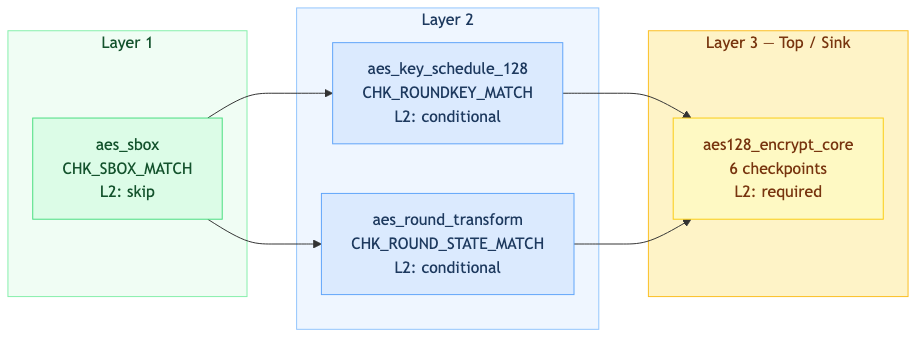
\includegraphics[keepaspectratio,alt={图 3-2: AES-128模块依赖DAG}]{../fpga_flow/diagrams/02_aes_node_dag.png}}
\caption{图 3-2: AES-128模块依赖DAG}
\end{figure}

4 个模块的角色与依赖关系如下：

\textbf{aes\_sbox（S-box 替换模块）}：实现 AES
标准中的字节替换操作，为纯组合逻辑，无上游依赖。该模块是 DAG
的叶节点（\texttt{integration\_role:\ leaf}），被
\texttt{aes\_key\_schedule\_128}、\texttt{aes\_round\_transform} 和
\texttt{aes128\_encrypt\_core}
三个模块依赖。由于其功能单一且无依赖，\texttt{l2\_policy} 设置为
\texttt{skip}（跳过鲁棒性测试）。

\textbf{aes\_key\_schedule\_128（密钥扩展模块）}：实现 AES-128
的密钥扩展算法，生成 11 组轮密钥（含初始密钥在内）。该模块依赖
\texttt{aes\_sbox}（用于 SubWord 操作），\texttt{l2\_policy} 为
\texttt{conditional}，\texttt{criticality} 为 \texttt{high}。

\textbf{aes\_round\_transform（轮变换模块）}：实现 AES 单轮的 4
步变换：SubBytes（字节替换）、ShiftRows（行移位）、MixColumns（列混合，基于
GF(2\^{}8) 有限域运算）和 AddRoundKey（轮密钥异或）。该模块依赖
\texttt{aes\_sbox}，\texttt{l2\_policy} 为
\texttt{conditional}，\texttt{criticality} 为 \texttt{high}。

\textbf{aes128\_encrypt\_core（顶层加密核心）}：实现 AES-128
加密的顶层有限状态机（FSM），集成上述全部子模块，实现 11 周期延迟（初始
AddRoundKey 1 周期 + 10 轮迭代各 1 周期）的 block-level handshake
接口。该模块是 DAG 的 sink
节点（\texttt{integration\_role:\ sink}），\texttt{l2\_policy} 为
\texttt{required}，\texttt{criticality} 为
\texttt{high}，是集成回归测试的顶层目标。

\subsubsection{3.2.2
模块端口规范}\label{ux6a21ux5757ux7aefux53e3ux89c4ux8303}

\textbf{表 3-2: 4 模块端口规范一览表}

{\def\LTcaptype{none} % do not increment counter
\begin{longtable}[]{@{}
  >{\raggedright\arraybackslash}p{(\linewidth - 8\tabcolsep) * \real{0.1875}}
  >{\raggedright\arraybackslash}p{(\linewidth - 8\tabcolsep) * \real{0.2500}}
  >{\raggedright\arraybackslash}p{(\linewidth - 8\tabcolsep) * \real{0.1875}}
  >{\raggedright\arraybackslash}p{(\linewidth - 8\tabcolsep) * \real{0.1875}}
  >{\raggedright\arraybackslash}p{(\linewidth - 8\tabcolsep) * \real{0.1875}}@{}}
\toprule\noalign{}
\begin{minipage}[b]{\linewidth}\raggedright
模块
\end{minipage} & \begin{minipage}[b]{\linewidth}\raggedright
信号名
\end{minipage} & \begin{minipage}[b]{\linewidth}\raggedright
方向
\end{minipage} & \begin{minipage}[b]{\linewidth}\raggedright
宽度
\end{minipage} & \begin{minipage}[b]{\linewidth}\raggedright
说明
\end{minipage} \\
\midrule\noalign{}
\endhead
\bottomrule\noalign{}
\endlastfoot
aes\_sbox & in\_byte & input & 8 & 待替换的输入字节 \\
aes\_sbox & out\_byte & output & 8 & 替换后的输出字节 \\
aes\_key\_schedule\_128 & key & input & 128 & AES-128 原始密钥 \\
aes\_key\_schedule\_128 & round\_keys & output & 1408 & 11
组轮密钥（11×128 bit） \\
aes\_round\_transform & state\_in & input & 128 & 轮变换输入状态 \\
aes\_round\_transform & round\_key & input & 128 & 本轮密钥 \\
aes\_round\_transform & is\_last\_round & input & 1 & 末轮标志（跳过
MixColumns） \\
aes\_round\_transform & state\_out & output & 128 & 轮变换输出状态 \\
aes128\_encrypt\_core & clk & input & 1 & 时钟信号 \\
aes128\_encrypt\_core & rst & input & 1 & 同步复位（高有效） \\
aes128\_encrypt\_core & start & input & 1 & 加密启动握手信号 \\
aes128\_encrypt\_core & plaintext & input & 128 & 明文输入 \\
aes128\_encrypt\_core & key & input & 128 & 加密密钥 \\
aes128\_encrypt\_core & ciphertext & output & 128 & 密文输出 \\
aes128\_encrypt\_core & done & output & 1 & 完成单周期脉冲 \\
aes128\_encrypt\_core & busy & output & 1 & 运算进行中标志 \\
\end{longtable}
}

上述接口规范在 \texttt{synthesis.py} 的 \texttt{\_aes\_blueprints()}
中以 \texttt{PortSpec} 字典形式定义，经
\texttt{ContractCompiler.compile\_module\_contract()} 转换为
\texttt{ModuleContract} 模型，并写入各模块工作区的
\texttt{module\_contract.json} 文件，成为 Agent
在生成和修复过程中不得更改的冻结接口约束。

\begin{center}\rule{0.5\linewidth}{0.5pt}\end{center}

\subsection{3.3 Agent 角色与 LLM
配置}\label{agent-ux89d2ux8272ux4e0e-llm-ux914dux7f6e}

\subsubsection{3.3.1 Agent
角色体系}\label{agent-ux89d2ux8272ux4f53ux7cfb}

本框架共定义 3 种 Agent 角色（由 \texttt{AgentRole} 枚举列出），对应 5
个 Agent 构建函数。\texttt{policy.py} 中的 \texttt{AgentRole}
枚举包含三个值：\texttt{WORKFLOW\_ORCHESTRATOR}（工作流编排器）、\texttt{MODULE\_WORKER\_SUBAGENT}（模块工作者子代理）和
\texttt{L2\_CAMPAIGN\_SUBAGENT}（L2
测试活动子代理）。\texttt{agents/specs.py} 中共提供 5
个构建函数：\texttt{build\_workflow\_orchestrator\_spec()} 和
\texttt{build\_finalizer\_orchestrator\_spec()} 均对应
\texttt{WORKFLOW\_ORCHESTRATOR}
角色（终态编排器复用编排器角色类型但使用不同的 LLM Profile
和工具集）；\texttt{build\_module\_worker\_spec()} 和
\texttt{build\_repair\_worker\_spec()} 均对应
\texttt{MODULE\_WORKER\_SUBAGENT}
角色（修复工作者复用模块工作者角色类型但不持有 \texttt{run\_executor}
工具）；\texttt{build\_l2\_campaign\_spec()} 对应
\texttt{L2\_CAMPAIGN\_SUBAGENT} 角色。每个构建函数返回的
\texttt{AgentSpawnSpec} 包含角色类型、LLM Profile、系统提示词、Skill
键集合、允许的编排器状态集合及可写路径约束。

具体来看，本框架设计了 5 个 Agent 构建函数：

\begin{itemize}
\tightlist
\item
  \texttt{build\_workflow\_orchestrator\_spec()}：构建执行编排器，使用
  \texttt{DEEPSEEK\_OFFICIAL\_FAST} profile，持有 \texttt{run\_executor}
  自定义工具，允许在除 \texttt{DONE} 之外的全部 9
  个状态下活动，不持有任何可写路径（编排器不直接写文件）。
\item
  \texttt{build\_finalizer\_orchestrator\_spec()}：构建终态汇总编排器，使用
  \texttt{DEEPSEEK\_OFFICIAL\_THINKING} profile，持有
  \texttt{FinishTool}，仅允许在
  \texttt{INTEGRATION\_READY}、\texttt{INTEGRATION\_REGRESSION}、\texttt{DONE}
  三个状态下活动，负责生成最终工作流报告后调用 \texttt{finish()}。
\item
  \texttt{build\_module\_worker\_spec(node)}：构建单模块工作者，使用
  \texttt{DEEPSEEK\_OFFICIAL\_FAST} profile，持有 \texttt{run\_executor}
  工具，可写路径严格限定为该节点的 RTL 文件和测试台文件，仅允许在
  \texttt{MODULE\_DESIGN}、\texttt{MODULE\_L0}、\texttt{MODULE\_L1}
  三个状态下活动。
\item
  \texttt{build\_repair\_worker\_spec()}：构建专用修复工作者，使用
  \texttt{DEEPSEEK\_OFFICIAL\_FAST} profile，不持有
  \texttt{run\_executor}（修复阶段不允许触发执行），遵循''编辑优先''协议。
\item
  \texttt{build\_l2\_campaign\_spec(node,\ ...)}：构建 L2
  测试活动代理，使用 \texttt{DEEPSEEK\_OFFICIAL\_FAST} profile，持有
  \texttt{run\_executor} 工具，仅允许在 \texttt{MODULE\_L2\_OPTIONAL}
  状态下活动，不允许 RTL 或测试台编辑。
\end{itemize}

\subsubsection{3.3.2 双 LLM Profile
策略}\label{ux53cc-llm-profile-ux7b56ux7565}

系统采用 \texttt{LLMProfileName} 枚举定义两种 DeepSeek API 调用配置：

\begin{itemize}
\tightlist
\item
  \texttt{DEEPSEEK\_OFFICIAL\_THINKING}（深度思考模式，\texttt{reasoning\_effort=\textquotesingle{}medium\textquotesingle{}}）：计算成本较高但推理能力强，用于需要跨模块推理的编排器（规格分析、架构设计、集成回归阶段）以及最终汇总编排器。
\item
  \texttt{DEEPSEEK\_OFFICIAL\_FAST}（快速执行模式，\texttt{reasoning\_effort=\textquotesingle{}none\textquotesingle{}}）：响应快速、成本低，用于局部任务执行的工作者（模块生成、验证、修复、L2
  测试）。
\end{itemize}

这一双 Profile
设计的核心逻辑是：跨模块决策（如判断模块间接口是否一致、决定是否升级）需要深度推理能力，而节点本地任务（如基于已有参考代码修复一个编译错误）不需要耗费推理资源，使用快速模式即可完成。通过在正确的任务上使用正确的
Profile，系统在保证决策质量的同时控制了 API 调用成本。

\textbf{表 3-3: Agent 角色-LLM Profile-工具矩阵}

{\def\LTcaptype{none} % do not increment counter
\begin{longtable}[]{@{}
  >{\raggedright\arraybackslash}p{(\linewidth - 6\tabcolsep) * \real{0.2444}}
  >{\raggedright\arraybackslash}p{(\linewidth - 6\tabcolsep) * \real{0.2889}}
  >{\raggedright\arraybackslash}p{(\linewidth - 6\tabcolsep) * \real{0.2000}}
  >{\raggedright\arraybackslash}p{(\linewidth - 6\tabcolsep) * \real{0.2667}}@{}}
\toprule\noalign{}
\begin{minipage}[b]{\linewidth}\raggedright
Agent 角色
\end{minipage} & \begin{minipage}[b]{\linewidth}\raggedright
LLM Profile
\end{minipage} & \begin{minipage}[b]{\linewidth}\raggedright
持有工具
\end{minipage} & \begin{minipage}[b]{\linewidth}\raggedright
典型活动状态
\end{minipage} \\
\midrule\noalign{}
\endhead
\bottomrule\noalign{}
\endlastfoot
执行编排器（Workflow Orchestrator） & FAST & run\_executor &
MODULE\_DESIGN / L0 / L1 \\
终态编排器（Finalizer Orchestrator） & THINKING & FinishTool &
INTEGRATION\_READY / DONE \\
模块工作者（Module Worker） & FAST & run\_executor & MODULE\_DESIGN / L0
/ L1 \\
修复工作者（Repair Worker） & FAST & 无 & MODULE\_DESIGN / L0 / L1 \\
L2 测试代理（L2 Campaign） & FAST & run\_executor &
MODULE\_L2\_OPTIONAL \\
\end{longtable}
}

\begin{center}\rule{0.5\linewidth}{0.5pt}\end{center}

\subsection{3.4 DAG
拓扑批调度与并行执行}\label{dag-ux62d3ux6251ux6279ux8c03ux5ea6ux4e0eux5e76ux884cux6267ux884c}

\subsubsection{3.4.1
拓扑分层算法}\label{ux62d3ux6251ux5206ux5c42ux7b97ux6cd5}

DAG 拓扑批调度是本框架处理多模块硬件设计的通用机制------对于任何 DAG
可分解的设计，\texttt{DAGBatchPlanner}
均可自动计算拓扑层级和并行批次。以下以 AES-128 的 4 节点 DAG
为具体示例说明其工作原理。

\texttt{synthesis.py} 中的 \texttt{DAGBatchPlanner} 类实现了基于 Kahn
算法变体的拓扑分层调度。\texttt{\_topological\_layers()}
方法计算每个节点的入度（依赖数量），将入度为 0
的节点放入初始就绪集合，按批次执行并在每次执行后将新满足依赖的节点加入下一批次。

对于 AES-128 的 4 节点 DAG，拓扑分层的结果为：

\begin{itemize}
\tightlist
\item
  \textbf{第一批次（Layer
  1）}：\texttt{{[}aes\_sbox{]}}------无依赖，单独执行。
\item
  \textbf{第二批次（Layer
  2）}：\texttt{{[}aes\_key\_schedule\_128,\ aes\_round\_transform,\ aes128\_encrypt\_core{]}}------在
  \texttt{aes\_sbox}
  完成后，三个模块的依赖均已满足，理论上可并行委派执行。
\end{itemize}

节点在同层内按优先级排序：首先按
\texttt{integration\_role}（\texttt{top} \textgreater{} \texttt{sink}
\textgreater{} \texttt{leaf} \textgreater{} \texttt{support}），其次按
\texttt{criticality}（\texttt{high} \textgreater{} \texttt{medium}
\textgreater{} \texttt{low}），最后按 \texttt{module\_id}
字母序。这一排序策略确保顶层/关键模块优先处理。

批次任务被封装为 \texttt{DelegateBatchPlan}，包含
\texttt{batch\_id}、\texttt{stage}（对应
\texttt{OrchestratorState}）、\texttt{max\_children}（最大子代理数，默认
5）和 \texttt{tasks} 列表。\texttt{max\_children}
限制了单批次并行子代理数量，防止对 LLM API 造成过大并发压力。

\begin{figure}
\centering
\pandocbounded{
\includegraphics[keepaspectratio,alt={图 3-3: 批次执行循环}]{../fpga_flow/diagrams/03_batch_execution_loop.png}}
\caption{图 3-3: 批次执行循环}
\end{figure}

\subsubsection{3.4.2
工作区生命周期状态机}\label{ux5de5ux4f5cux533aux751fux547dux5468ux671fux72b6ux6001ux673a}

每个节点的工作区存在独立的状态机，由 \texttt{NodeWorkspaceState}
枚举定义 7 个状态：

\begin{itemize}
\tightlist
\item
  \texttt{MISSING}：工作区尚未初始化
\item
  \texttt{DRAFT\_READY}：工作区已初始化、草稿文件已由 Memory 预填充
\item
  \texttt{VALIDATED}：L0 编译和 L1 仿真均通过，所有必需 Checkpoint 均为
  PASS
\item
  \texttt{PROMOTED}：已从草稿工作区晋升至规范 RTL/TB 路径
\item
  \texttt{REPAIRING}：验证失败，正在修复循环中（未超出预算）
\item
  \texttt{BLOCKED}：修复预算耗尽，需要人工介入或升级至思考型编排器
\item
  \texttt{FAILED}：发生不可恢复的错误
\end{itemize}

\texttt{NodePolicyEngine.decide\_next\_mode()} 根据当前
\texttt{NodeWorkspaceRecord} 状态和验证结果决定下一个
\texttt{SubagentWorkMode}（\texttt{GENERATE}、\texttt{VALIDATE}、\texttt{REPAIR}、\texttt{L2\_EXECUTE}
或 \texttt{INTEGRATION}）。这一决策逻辑完全在框架侧执行，LLM
无法直接影响工作区状态的推进。

\begin{center}\rule{0.5\linewidth}{0.5pt}\end{center}

\subsection{3.5
关键支撑机制概述}\label{ux5173ux952eux652fux6491ux673aux5236ux6982ux8ff0}

\subsubsection{3.5.1
结构化修复循环}\label{ux7ed3ux6784ux5316ux4feeux590dux5faaux73af}

当 L0 编译或 L1
仿真失败时，系统启动结构化修复循环。修复循环的完整流程为：

\begin{enumerate}
\def\labelenumi{\arabic{enumi}.}
\tightlist
\item
  \texttt{write\_repair\_request()} 生成 \texttt{RepairContract}
  并写入工作区，其中包含失败阶段（\texttt{failure\_phase}）、主要目标文件（\texttt{primary\_target\_file}）、文件片段（\texttt{primary\_file\_excerpt}）、错误摘要（\texttt{error\_excerpt}）、仿真日志摘要（\texttt{simulation\_log\_excerpt}）及第一步编辑指令（\texttt{first\_edit\_steps}）。
\item
  修复工作者 Agent 读取 \texttt{RepairContract}，按照
  \texttt{REPAIR\_PHASE\_ROUND\_1} 或
  \texttt{REPAIR\_PHASE\_ROUND\_2\_PLUS}
  阶段混入的约束执行精确编辑。第一轮修复的硬性要求是：\textbf{第一个工具调用必须是对
  \texttt{primary\_target\_file} 的文件编辑}，防止 Agent 偏离修复范围。
\item
  \texttt{verify\_repair\_edit()} 通过 SHA-256
  哈希比对验证文件确实发生了实质性变化，并检查
  \texttt{must\_add\_tokens}
  列表中的必要令牌是否已被添加。哈希验证失败意味着 Agent
  未实际修改文件，系统将拒绝该修复并记录失败。
\item
  \texttt{write\_edit\_receipt()} 写出
  \texttt{EditReceipt}，记录已编辑的文件列表和第一步编辑摘要。
\item
  重新触发 L0/L1 验证。
\end{enumerate}

\subsubsection{3.5.2 升级策略}\label{ux5347ux7ea7ux7b56ux7565}

\texttt{AgentExecutionPolicy.should\_escalate()}
是升级决策的唯一入口，当下列任一条件满足时返回 \texttt{True}：

\begin{itemize}
\tightlist
\item
  \texttt{repair\_attempts\ \textgreater{}=\ repair\_attempt\_threshold}（修复次数达到阈值，默认
  2 次）
\item
  \texttt{cross\_module\_issue=True}（问题跨越模块边界）
\item
  \texttt{state\_machine\_issue=True}（涉及状态机逻辑错误）
\item
  \texttt{interface\_issue=True}（涉及接口信号不兼容）
\end{itemize}

升级后，控制权从快速模式的工作者 Agent
返回至深度思考模式的编排器，携带完整的失败上下文（失败阶段、错误日志、已尝试的修复历史），由编排器决定后续策略（继续修复、放弃该节点或重新规划）。

\subsubsection{3.5.3 Pydantic
反幻觉机制}\label{pydantic-ux53cdux5e7bux89c9ux673aux5236}

所有合约模型均使用
\texttt{ConfigDict(extra=\textquotesingle{}forbid\textquotesingle{})}，这意味着任何
JSON 响应中出现的多余字段都会在反序列化时立即触发
\texttt{ValidationError}。结合 \texttt{@model\_validator}
中的范围约束（如 \texttt{SpecIR} 强制
\texttt{algorithm=\textquotesingle{}AES\textquotesingle{}}、\texttt{variant=\textquotesingle{}AES-128\textquotesingle{}}、\texttt{latency\_target\_cycles=11}），系统构建了一个机器可检查的约束体系，有效防止
LLM 幻觉污染核心数据结构。

\begin{center}\rule{0.5\linewidth}{0.5pt}\end{center}

本章从整体层面描述了框架的通用六层架构设计，并以 AES-128
验证案例展示了模块 DAG 分解、Agent 角色配置和 DAG
批调度的具体实例化。这一架构设计的核心优势在于：关注点分离（每层职责单一）、控制权内聚（框架而非
LLM
掌握进度判断）以及设计无关性（架构层面的通用性使其可适配不同的硬件设计目标）。后续各章将对状态机编排（第四章）、分层验证体系（第五章）和
LLM
约束引擎（第六章）三个核心创新点进行深入展开，每个创新点均先阐述通用设计原理，再以
AES-128 案例展示具体实例化。
